% !TEX root = doc.tex
% Copyright (c) 2017-2020 The ALF project.
% This is a part of the ALF project documentation.
% The ALF project documentation by the ALF contributors is licensed
% under a Creative Commons Attribution-ShareAlike 4.0 International License.
% For the licensing details of the documentation see license.CCBYSA.
%
%-----------------------------------------------------------------------------------


%-----------------------------------------------------------------------------------
\subsection{Generic hopping  matrices on Bravais lattices} \label{sec:predefined_hopping_1}
%-----------------------------------------------------------------------------------

The module \texttt{Predefined\_Hopping}   provides a   generic way to   specify a  hopping matrix on a  multi-orbital Bravais lattice.  The only  assumption that we make is  translation symmetry.   We   allow  for twisted  boundary conditions in the $\vec{L}_1$ and $\vec{L}_2$ lattice directions. The twist is given by  \texttt{Phi\_X}  and \texttt{Phi\_Y}  respectively.  If the flag  \texttt{bulk=.true.}, then the twist is implemented with a vector potential. Otherwise, if  \texttt{bulk=.false.}, the twist is imposed at the boundary. The routine also accounts for  the inclusion of a  total number of \texttt{N\_Phi}  flux quanta traversing the lattice.  All phase factors mentioned above can be flavor dependent.   Finally, the checkerboard decomposition can also be specified in this module.


%-----------------------------------------------------------------------------------
\subsubsection{Setting up the hopping matrix: the \texttt{Hopping\_Matrix\_type}}\label{sec:hopping_type}

All information for setting up a generic hopping matrix on a lattice, including the checkerboard decomposition, is specified in the  \path{Hopping_Matrix_type} type, which we describe in the remaining of this section. The information stored in this type (see Table~\ref{table:Hopping_matrix}) fully defines the array of  operator type \path{OP_T} that accounts for the single particle propagation in one time step, from which the kinetic energy can be derived as well.    

\paragraph*{Generic hopping matrices}\label{sec:generic_hopping}
%-----------------------------------------------------------------------------------

The generic Hopping Hamiltonian  reads: 
\begin{equation}
\hat{H}_T = \sum_{(i,\delta), (j,\delta'), s, \sigma}    T_{(i,\delta), (j,\delta')}^{(s)}    \hat{c}^{\dagger}_{(i,\delta),s,\sigma }   e^{\frac{2 \pi i}{\Phi_0} \int_{i + \delta}^{j + \delta'}  \vec{A}^{(s)}(\vec{l})  d \vec{l}} \hat{c}^{}_{(j,\delta'),s,\sigma }
\label{generic_hopping.eq}
\end{equation}
with boundary conditions 
\begin{equation}
\hat{c}^{\dagger}_{(i + L_i,\delta) ,s,\sigma }   =  e^{- 2 \pi i\frac{\Phi_i^{(s)}}{\Phi_0}} \, e^{\frac{2 \pi i }{\Phi_0} \chi^{(s)}_{L_i} ( i + \delta ) } \, \hat{c}^{\dagger}_{(i,\delta) ,s,\sigma }.
\label{generic_boundary.eq}
\end{equation}
Here $i$  labels the unit cell and $\delta$    the orbital.
Both the twist and  vector  potential can have a flavor dependency. These and the other components of the generic Hopping Hamiltonian are described bellow. For now onwards we will  mostly omit the flavor index ${s}$.\\

\noindent
\textbf{Phase factors}.  
The vector potential accounts for an orbital magnetic field in the $z$ direction that is implemented  in the Landau  gauge:  $\vec{A}(\vec{x})  =  -B(y,0,0) $ with $ \vec{x} = (x,y,z)$. $\Phi_0$ corresponds to the flux quanta and the scalar function $\chi$ is defined through:
\begin{equation}
\vec{A}( \vec{x} + \vec{L}_{i} )  = \vec{A}( \vec{x} )   +  \vec{\nabla} \chi_{L_{i}}(\vec{x}). 
\end{equation}

Provided that the bare hopping Hamiltonian, $T$ (i.e., without phases, see Eq.~\eqref{eq:hop}), is invariant under lattice translations, $\hat{H}_T$ commutes with magnetic translations that satisfy the algebra:
\begin{equation}
\hat{T}_{\vec{a}} \hat{T}_{\vec{b}} =  e^{ \frac{2 \pi i}{\Phi_0}   \vec{B} \cdot \left( \vec{a} \times \vec{b} \right) }  \hat{T}_{\vec{b}} \hat{T}_{\vec{a}}. 
\end{equation}
On the  torus, the uniqueness of the wave functions requires that  $\hat{T}_{\vec{L}_1} \hat{T}_{\vec{L}_2}  =   \hat{T}_{\vec{L}_2} \hat{T}_{\vec{L}_1} $ such
that
\begin{equation}
\frac{\vec{B} \cdot \left( \vec{a} \times \vec{b}  \right) }{\Phi_0 } = N_{\Phi}   
\end{equation}
with  $N_\Phi $ an integer.  The variable \texttt{N\_Phi},   specified in the parameter file,   denotes the number of flux quanta piercing the lattice.    The variables \texttt{Phi\_X}  and   \texttt{Phi\_Y} also   in the parameter file denote  the twists  -- in units of the flux quanta  --  along the $\vec{L}_1$ and  $\vec{L}_2$ directions.     There are gauge  equivalent ways to insert the  twist in the boundary conditions. In the above we  have inserted the twist as a boundary condition such that for example setting \texttt{Phi\_1=0.5}  corresponds to anti-periodic boundary conditions along the $L_1$  axis.
Alternatively we can consider the Hamiltonian:
\begin{equation}
\hat{H}_T = \sum_{(i,\delta), (j,\delta'), s, \sigma}    T_{(i,\delta), (j,\delta')}^{(s)}    \tilde{c}^{\dagger}_{(i,\delta),s,\sigma }   e^{\frac{2 \pi i}{\Phi_0} \int_{i + \delta}^{j + \delta'} \left(  \vec{A}(\vec{l})  + \vec{A}_{\phi} \right)  d \vec{l}} \tilde{c}^{}_{(j,\delta'),s,\sigma }
\end{equation}
with boundary conditions 
\begin{equation}
\tilde{c}^{\dagger}_{(i + L_i,\delta) ,s,\sigma }   =  e^{\frac{2 \pi i }{\Phi_0} \chi_{L_i} ( i + \delta ) } \, \tilde{c}^{\dagger}_{(i,\delta) ,s,\sigma }.
\end{equation}
Here 
\begin{equation}
\vec{A}_{\phi} =\frac{  \phi_1  |\vec{a}_1|} { 2 \pi |\vec{L}_1| } \vec{b}_1 +  \frac{  \phi_2  |\vec{a}_2|}{2 \pi  |\vec{L}_2| } \vec{b}_2
\end{equation}
and $\vec{b}_i$  corresponds to the reciprocal lattice vectors satisfying  $ \vec{a}_i  \cdot  \vec{b}_j  = 2 \pi \delta_{i,j} $.   The logical variable $\texttt{bulk} $ chooses between these two  gauge equivalent ways  of inserting the twist angle. If \texttt{bulk=.true.} then  we use periodic boundary conditions  --  in the absence of an orbital field -- otherwise  twisted boundaries are used.  
The above phase factors are computed  in the   module function: 
\begin{lstlisting}[style=fortran]
complex function Generic_hopping(i, no_i, n_1, n_2, no_j, N_Phi, Phi_1, Phi_2, Bulk, 
                                 Latt, Latt_Unit)
\end{lstlisting}
which returns the  phase factor involved in the hopping of a hole from lattice site $ \ve{i} + \ve{\delta}_{\text{no}_i} $ to 
$\ve{i} + n_1 \ve{a}_1 + n_2 \ve{a}_2+ \ve{\delta}_{\text{no}_j}  $.  Here  $\ve{\delta}_{\text{no}_i}$  is  the position of the $\text{no}_i$  orbital in the unit cell
$\ve{i}$. 
The information for the phases is encoded in the type \texttt{Hopping\_matrix\_type}.\\

\noindent
\textbf{The  Hopping matrix elements}. 
The hopping matrix  is specified assuming only translation invariance.  (The point group symmetry of the lattice can be broken.)
That is, we assume that  for  each flavor index:
\begin{equation} 
T_{(\ve{i},\,\ve{\delta}), (\ve{i} +  n_1\vec{a}_1  + n_2 \vec{a}_2,\,\ve{\delta}')}^{(s)}   =   T^{(s)}_{(\ve{0},\,\ve{\delta}),  (n_1\vec{a}_1  + n_2 \vec{a}_2,\,\ve{\delta}') }.
\label{eq:hop}	 
\end{equation}
The right  hand side of the above equation is given  the type  \texttt{Hopping\_matrix\_type}.\\


\noindent
\textbf{The checkerboard decomposition.}   Aside from the hopping phases and hopping matrix elements, the \texttt{Hopping\_matrix\_type} type contains information  concerning the checkerboard   decomposition.  In Eq.~\eqref{Checkerboard.Eq} we wrote the hopping Hamiltonian as:
\begin{equation}
\hat{\mathcal{H}}_{T}     = \sum_{i=1}^{N_T} \sum_{k \in \mathcal{S}^{T}_i} \hat{T}^{(k)},  
\end{equation}
with the rule that  if $k$ and $k'$  belong to the same set $\mathcal{S}^{T}_i $ then   $ \big[ \hat{T}^{(k)} , \hat{T}^{(k')} \big] = 0 $.  In the checkerboard decomposition, $\hat{T}^{(k)}$   corresponds to  hopping on a bond.    The checkerboard decomposition depends on the   lattice type, as well as on the hopping matrix elements.   The required  information is stored in  \texttt{Hopping\_matrix\_type}. In this data type,  \texttt{N\_FAM}  corresponds to the number of sets  (or families) ($N_T$ in the above equation). \texttt{L\_FAM(1:N\_FAM)}   corresponds to the number of bonds in the set,  and finally,  \texttt{LIST\_FAM(1:N\_FAM, 1:max(L\_FAM(:)), 2)}    contains  information concerning the two legs of the bonds.    In the checkerboard decomposition, care has to be taken for local terms: each site  occurs multiple times in the list of bonds.    Since we have postulated translation symmetry,    a one-dimensional array, \texttt{Multiplicity},  of length  given by  the number of orbitals per unit cell suffices to  encode the required information.  
Finally, to be able to generate  the imaginary time step of length $\Delta \tau$  we  have to know   by which fraction of  $\Delta \tau$   we have to propagate each set.  This information is given in  the array  \texttt{Prop\_Fam}.  

As an  example we can consider the three-leg ladder lattice of Figure~\ref{fig_predefined_lattices}(c).   Here the number of sets (or families) \texttt{N\_FAM} is equal to four, corresponding to the red, green, black and blue  bonds. It is clear from the figure that bonds in a given set do not have common legs, so that hopping instances on the bonds of a given set commute.  For this three-leg ladder, we see that the middle orbital in a unit cell appears in each set or family. It hence has a multiplicity of four. On the other hand, the top and bottom orbitals have a multiplicity of 3 since they appear in only three of the four sets. 


\paragraph*{Usage: the \texttt{Hopping\_Matrix\_type} } %\label{Hopping_Matrix_type.sec} 

There are \path{N_bonds} hopping matrix elements emanating from a given unit cell, defined so that looping over all of the elements does not overcount the bonds. For each bond, the array 
\texttt{List}   contains the full  information to define the  RHS of Eq.~\eqref{eq:hop}.    The hopping amplitudes are  stored in the  array  \texttt{T}  and the local potentials in the  array \texttt{T\_loc}   (See  Table~\ref{table:Hopping_matrix}).    The  \texttt{Hopping\_Matrix\_type}   type    also contains the information for the  checkerboard   decomposition.

\begin{table}[h]
	\begin{center}
		%    \begin{tabular}{@{} l l l @{}}\toprule
		\begin{tabular}{@{} p{0.42\columnwidth} @{} p{0.09\columnwidth} p{0.46\columnwidth} @{}}\toprule
			Variable                 & Type            & Description \\\midrule
			\texttt{N\_bonds}        & \texttt{int}    & Number of  hopping  matrix elements within and  emanating from   a unit cell   \\
			\texttt{List(N\_bonds,4)}& \texttt{int}    & List($\bullet$,1) =   $\delta$ \\
			&                 & List($\bullet$,2) =   $\delta'$ \\
			&                 & List($\bullet$,3) =   $n_1$     \\
			&                 & List($\bullet$,4) =   $n_2$     \\ 
			\texttt{T(N\_bonds)}     & \texttt{cmplx}  & Hopping amplitude   \\
			\texttt{T\_loc(Norb)}    & \texttt{cmplx}  & On site  potentials (e.g., chemical potential, Zeeman field)   \\
			\texttt{N\_Phi}          & \texttt{int}    & Number of  flux quanta piercing the lattice   \\
			\texttt{Phi\_X}          & \texttt{dble}   & Twist in $\ve{a}_1$  direction   \\
			\texttt{Phi\_Y}          & \texttt{dble}   & Twist in $\ve{a}_2$  direction   \\
			\texttt{Bulk}            & \texttt{logical}& Twist as vector potential (T) or  boundary condition (F)  \\
			\texttt{N\_Fam}          & \texttt{int}    & Number of  sets, $N_T$ in Eq.~\eqref{Checkerboard.Eq}   \\
			\texttt{L\_Fam(N\_FAM)}  & \texttt{int}    & Number of bonds per set $\mathcal{S}^{T}$ \\    
			\texttt{List\_Fam(N\_FAM,max(L\_FAM(:)),2)}& \texttt{int} & \texttt{List\_Fam($ \bullet,\bullet $,1)} =  Unit cell \\
			&                        &          \texttt{List\_Fam($\bullet,\bullet$,2)} =   Bond number \\
			\texttt{Multiplicity(Norb)}& \texttt{int}  & Number of  times a  given orbital  occurs in the list of bonds  \\
			\texttt{Prop\_Fam(N\_FAM)} & \texttt{dble}         & The fraction of $\Delta \tau$ with which the set will be propagated   \\\bottomrule
		\end{tabular}
		\caption{Member variables of the \texttt{Hopping\_Matrix\_type}  type.   
			\label{table:Hopping_matrix}}
	\end{center}
\end{table}

The  data in the \texttt{Hopping\_matrix\_type} type suffices to uniquely define the  unit step propagation for the kinetic energy, and for  any combinations of the  \texttt{Checkerboard} and  \texttt{Symm}  options (see Sec.~\ref{sec:trotter}). The propagation is set through the call: 
\begin{lstlisting}[style=fortran]
Call Predefined_Hoppings_set_OPT(Hopping_Matrix, List, Invlist, Latt, Latt_unit, Dtau,
                                 Checkerboard, Symm, OP_T)
\end{lstlisting}
in which the operator array \path{OP_T(*,N_FL)} is allocated and defined. In the simplest case, where no checkerboard is used, the array's first dimension is unity.


The   data in  the \texttt{Hopping\_matrix\_type} type   equally  suffices to compute  the kinetic energy.  This is carried out in the routine \texttt{Predefined\_Hoppings\_Compute\_Kin}.

\subsubsection{An example:   nearest neighbor hopping on the   honeycomb lattice }

\begin{figure}
	\begin{center}
		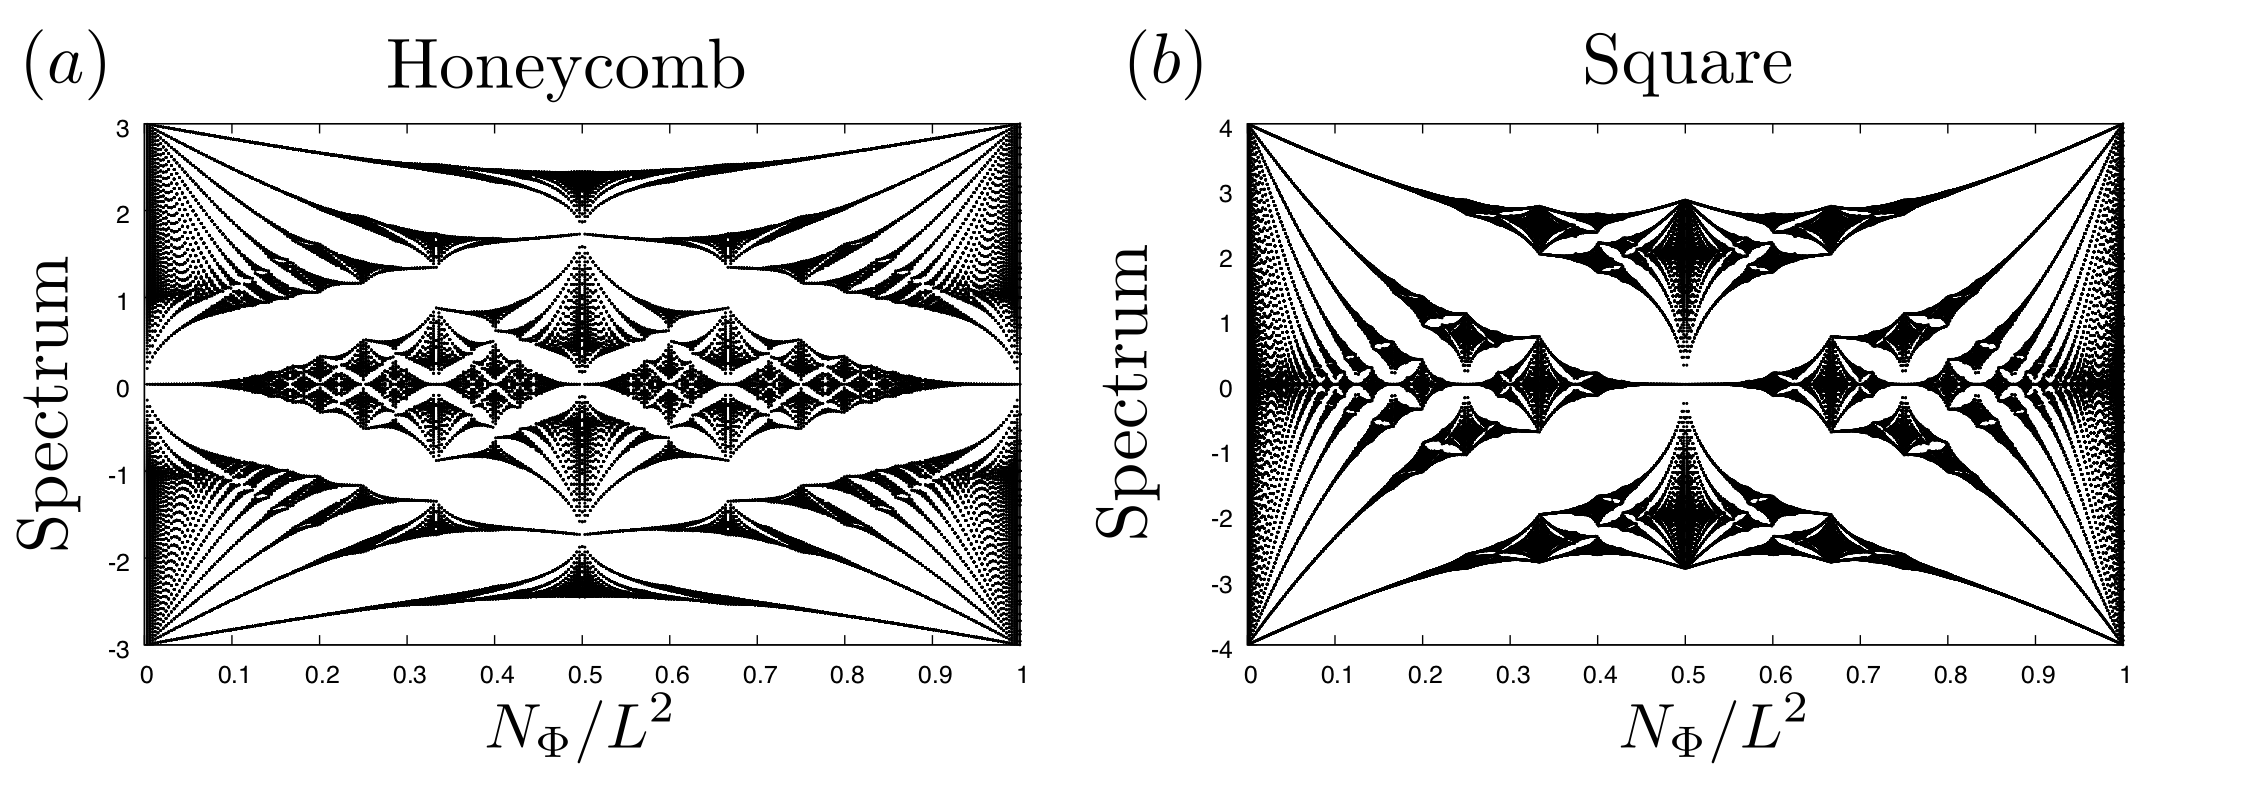
\includegraphics[width=0.95\textwidth,clip]{But.png}
		\caption{The single particle spectrum  of the tight binding model on the  honeycomb  (a) and square (b) lattices as a function of the  flux  $N_\Phi$.    This corresponds to the well known  Hofstadter butterflies.  }
		\label{But.fig}
	\end{center}
\end{figure}

For the honeycomb lattice of  Fig.~\ref{fig_predefined_lattices}(d)   the number of  bond within and emanating from  a unit cell is \texttt{N\_bonds = 3}.     The list array of the \texttt{Hopping\_matrix\_type} reads:

\begin{lstlisting}[style=fortran,escapechar=\#]
list(1,1) = 1;  list(1,2) = 2;  list(1,3) = 0;   list(1,4) =  0 ! Intra unit-cell hopping
list(2,1) = 2;  list(2,2) = 1;  list(2,3) = 0:   list(2,4) =  1 ! Inter unit-cell hopping
list(3,1) = 1;  list(3,2) = 2;  list(3,3) = 1:   list(3,4) = -1 ! Inter unit-cell hopping
T(1) = -1.0;  T(2) = -1.0;  T(3) = -1.0                         ! Hopping
T_loc(1) = 0.0;  T_loc(2) = 0.0                                 ! Chemical potential 
\end{lstlisting} 
In the last two lines, we have set the hopping matrix element  for each bond to $-1$  and the chemical potential to zero.    The fields,   can then be specified   with the  variables   \texttt{N\_phi, Phi\_x, Phi\_y}.  Setting   the twists, 
\texttt{Phi\_x, Phi\_y}  to zero and  looping over \texttt{N\_phi}    from $ 1 \cdots L^2 $   produces  the single particle spectrum of  Fig.~\ref{But.fig}(a).  

For the honeycomb lattice  the checkerboard decomposition  for the nearest neighbor hopping consists of three  sets:  \texttt{N\_Fam = 3}  each of length   corresponding  to the number of unit cells.  In  Fig.~\ref{fig_predefined_lattices}(d)  
these sets are denoted by different colors. In the code, the elements of the sets are specified as:

\begin{lstlisting}[style=fortran] 
do I = 1,Latt%N
   do nf = 1,N_FAM
      List_Fam(nf,I,1) = I  ! Unit cell
      List_Fam(nf,I,2) = nf ! The bond 
   enddo
enddo
Multiplicity  = 3
\end{lstlisting}        
Since each site of the honeycomb lattice occurs in  the three sets, their multiplicity is equal to 3.  


%-----------------------------------------------------------------------------------
\subsubsection{Predefined hoppings}

The  module provides hopping and checkerboard decompositions, defining a  \path{Hopping_Matrix} (an array of length \path{N_FL} of type  \path{Hopping_Matrix_type}, see Sec.~\ref{sec:hopping_type}) for each of the following predefined lattices.

\subsubsection*{Square}
The call:
\begin{lstlisting}[style=fortran]
Call Set_Default_hopping_parameters_square(Hopping_Matrix, T_vec, Chem_vec, Phi_X_vec,  
         Phi_Y_vec, Bulk, N_Phi_vec, N_FL, List, Invlist, Latt, Latt_unit)
\end{lstlisting}
defines  the  \path{Hopping_Matrix} for the square  lattice: 
\begin{equation}
\hat{H}_T  =   \sum_{\ve{i}, \sigma, s}  \left( \left[ \sum_{ \ve{\delta} = \left\{ \ve{a}_1, \ve{a}_2\right\} }    - t^{(s)} \hat{c}^{\dagger}_{\ve{i},s,\sigma}   e^{\frac{2 \pi i}{\Phi_0} \int_{\ve{i}}^{\ve{i}+ \ve{\delta}}  \vec{A}^{(s)}(\vec{l})  d \vec{l}}   \hat{c}^{}_{\ve{i} + \ve{\delta},s,\sigma} +  \hc   \right]    -  \mu^{(s)} \hat{c}^{\dagger}_{\ve{i},s,\sigma} \hat{c}^{}_{\ve{i},s,\sigma}  \right).
\end{equation}
The vectors  \path{T_vec} and \path{Chem_vec} have  length \texttt{N\_FL} and specify the hopping and the chemical potentials, while the  vectors \path{Phi_X_vec},  \path{Phi_Y_vec} and \path{N_Phi_vec},  also of  length  \texttt{N\_FL},    define the vector potential. 


\subsubsection*{Honeycomb}
The call: 
\begin{lstlisting}[style=fortran]
Call Set_Default_hopping_parameters_honeycomb(Hopping_Matrix,T_vec, Chem_vec, Phi_X_vec,
         Phi_Y_vec, Bulk, N_Phi_vec, N_FL, List, Invlist, Latt, Latt_unit)
\end{lstlisting}
defines  the  \path{Hopping_Matrix} for the  honeycomb lattice: 
\begin{multline}
\hat{H}_T  =  \sum_{\ve{i}, \sigma, s}  \left(  \sum_{ \ve{\delta} = \left\{ \ve{\delta}_1, \ve{\delta}_2, \ve{\delta}_3\right\} }    - t^{(s)} \hat{c}^{\dagger}_{\ve{i},s,\sigma}   e^{\frac{2 \pi i}{\Phi_0} \int_{\ve{i}}^{\ve{i}+ \ve{\delta}}  \vec{A}^{(s)}(\vec{l})  d \vec{l}}   \hat{c}^{}_{\ve{i} + \ve{\delta},s,\sigma} +  \hc \right)   \\   
    +  \sum_{\ve{i}, \sigma, s}   -  \mu^{(s)} \left( \hat{c}^{\dagger}_{\ve{i},s,\sigma} \hat{c}^{}_{\ve{i},s,\sigma}   +  \hat{c}^{\dagger}_{\ve{i} + \ve{\delta}_1,s,\sigma} \hat{c}^{}_{\ve{i} + \ve{\delta}_1,s,\sigma}   \right),
\end{multline}
where the \path{T_vec} and \path{Chem_vec} have  length \texttt{N\_FL} and specify the hopping and the chemical potentials, while the  vectors \path{Phi_X_vec},  \path{Phi_Y_vec} and \path{N_Phi_vec},  also of  length  \texttt{N\_FL}, define the vector potential.  Here $\ve{i}$  runs over  sublattice  A, and $\ve{i} + \ve{\delta}$  over the three nearest neighbors of site $\ve{i}$.


\subsubsection*{Square bilayer}
The call:
\begin{lstlisting}[style=fortran]
Call Set_Default_hopping_parameters_Bilayer_square(Hopping_Matrix, T1_vec, T2_vec,
         Tperp_vec, Chem_vec, Phi_X_vec, Phi_Y_vec, Bulk, N_Phi_vec, N_FL, List, Invlist,
         Latt, Latt_unit)
\end{lstlisting}  
defines  the  \path{Hopping_Matrix} for the  bilayer  square  lattice:       
\begin{multline}
\hat{H}_T  =    \sum_{\ve{i}, \sigma, s,n } \left(    \left[  \sum_{ \ve{\delta} = \left\{ \ve{a}_1, \ve{a}_2\right\} } \!\! - t_n^{(s)} \hat{c}^{\dagger}_{\ve{i},s,\sigma,n}   e^{\frac{2 \pi i}{\Phi_0} \int_{\ve{i}}^{\ve{i}+ \ve{\delta}}  \vec{A}^{(s)}(\vec{l})  d \vec{l}}   \hat{c}^{}_{\ve{i} + \ve{\delta},s,\sigma,n} +  \hc \right]       -  \mu^{(s)} \hat{c}^{\dagger}_{\ve{i},s,\sigma,n} \hat{c}^{}_{\ve{i},s,\sigma,n}  \right)   \\
     + \sum_{\ve{i}, \sigma, s } -  t_{\perp}^{(s)}  \left( \hat{c}^{\dagger}_{\ve{i},s,\sigma,1} \hat{c}^{}_{\ve{i},s,\sigma,2}  + \hc \right), 
\end{multline}
where the additional  index  $n$  labels the layers.


\subsubsection*{Honeycomb  bilayer}
The call:
\begin{lstlisting}[style=fortran]
Call Set_Default_hopping_parameters_Bilayer_honeycomb(Hopping_Matrix, T1_vec, T2_vec,
         Tperp_vec, Chem_vec, Phi_X_vec, Phi_Y_vec, Bulk, N_Phi_vec, N_FL, List, Invlist,
         Latt, Latt_unit)
\end{lstlisting}  
defines  the  \path{Hopping_Matrix} for the  bilayer  honeycomb  lattice:                 
\begin{align}
\hat{H}_T  =  &   \sum_{\ve{i}, \sigma, s,n } \left(  \sum_{ \ve{\delta} = \left\{ \ve{\delta}_1, \ve{\delta}_2, \ve{\delta}_3 \right\} }  - t_n^{(s)} \hat{c}^{\dagger}_{\ve{i},s,\sigma,n}   e^{\frac{2 \pi i}{\Phi_0} \int_{\ve{i}}^{\ve{i}+ \ve{\delta}}  \vec{A}^{(s)}(\vec{l})  d \vec{l}}   \hat{c}^{}_{\ve{i} + \ve{\delta},s,\sigma,n} +  \hc \right)       \nonumber \\
      & +   \sum_{\ve{i}, \sigma, s } -  t_{\perp}^{(s)}  \left( \hat{c}^{\dagger}_{\ve{i},s,\sigma,1} \hat{c}^{}_{\ve{i},s,\sigma,2}   +
                   \hat{c}^{\dagger}_{\ve{i} + \ve{\delta}_1,s,\sigma,1} \hat{c}^{}_{\ve{i} + \ve{\delta}_1,s,\sigma,2}  + \hc  \right)   \nonumber \\
      & +   \sum_{\ve{i}, \sigma, s, n }  -  \mu^{(s)}  \left(\hat{c}^{\dagger}_{\ve{i},s,\sigma,n} \hat{c}^{}_{\ve{i},s,\sigma,n}  +  \hat{c}^{\dagger}_{\ve{i} + \ve{\delta}_1,s,\sigma,n} \hat{c}^{}_{\ve{i} + \ve{\delta}_1 ,s,\sigma,n}  \right)  
\end{align}
Here, the additional  index  $n$  labels the layer.   $\ve{i} $   runs over the unit cells  and   $\ve{\delta} = \left\{ \ve{\delta}_1, \ve{\delta}_2, \ve{\delta}_3 \right\} $  over the three nearest neighbors. 


\subsubsection*{N-leg ladder}
The call:
\begin{lstlisting}[style=fortran]
Call Set_Default_hopping_parameters_n_lag_ladder(Hopping_Matrix, T_vec, Tperp_vec,
    Chem_vec, Phi_X_vec, Phi_Y_vec, Bulk, N_Phi_vec, N_FL, List, Invlist, Latt, Latt_unit)
\end{lstlisting}  
defines  the  \path{Hopping_Matrix} for the  the  N-leg ladder lattice:                 
\begin{multline}
\hat{H}_T  =  \sum_{\ve{i}, \sigma, s }  \sum_{n=1}^{\texttt{Norb}} \left(      - t^{(s)} \hat{c}^{\dagger}_{\ve{i},s,\sigma,n}   e^{\frac{2 \pi i}{\Phi_0} \int_{\ve{i}}^{\ve{i}+ \ve{a}_1}  \vec{A}^{(s)}(\vec{l})  d \vec{l}}   \hat{c}^{}_{\ve{i} + \ve{a}_1,s,\sigma,n} +  \hc       -  \mu^{(s)} \hat{c}^{\dagger}_{\ve{i},s,\sigma,n} \hat{c}^{}_{\ve{i},s,\sigma,n}  \right)    \\
     + \sum_{\ve{i}, \sigma, s } \sum_{n=1}^{\texttt{Norb}-1}  -  t_{\perp}^{(s)}  \left( 
                   \hat{c}^{\dagger}_{\ve{i} + \ve{\delta}_1,s,\sigma,n}  e^{\frac{2 \pi i}{\Phi_0} \int_{(n-1)\ve{a}_2}^{(n)\ve{a}_2}  \vec{A}^{(s)}(\vec{l})  d \vec{l}}    \hat{c}^{}_{\ve{i} + \ve{\delta}_1,s,\sigma,n+1}  + \hc  \right). 
\end{multline}
Here, the additional  index  $n$  defines  the orbital.  Note that this lattice  has open boundary conditions in the $\vec{a}_2$  direction. 
